\documentclass[5p,times]{elsarticle}

\usepackage{amsmath,amssymb,amsthm}
\usepackage{booktabs,multirow,tabularx,threeparttable}
\usepackage{graphicx}
\usepackage{xcolor}
\usepackage{algorithm}
\usepackage{algpseudocode}
\usepackage{tikz}
\usetikzlibrary{arrows.meta,positioning,fit,calc}
\usepackage{microtype}
\usepackage{xspace}
\usepackage[colorlinks=true,linkcolor=blue,citecolor=blue,urlcolor=blue]{hyperref}
\setlength{\emergencystretch}{1.2em}

\newtheorem{definition}{Definition}
\newtheorem{proposition}{Proposition}
\newtheorem{theorem}{Theorem}
\newtheorem{remark}{Remark}

\newcommand{\ledger}{\textsc{Ledger}\xspace}
\newcommand{\cl}{\operatorname{Cl}}
\newcommand{\tol}{\varepsilon}
\newcommand{\opset}{\mathcal{O}}
\newcommand{\operands}{\Omega}
\newcommand{\cert}{\mathsf{cert}}
\newcommand{\unknown}{\mathsf{unknown}}
\newcommand{\failure}{\mathsf{failure}}
\newcommand{\etitle}[1]{%
  \par\vspace{0.35ex}\noindent\textbf{\textit{#1}}\hspace{0.4em}}

\journal{Information Processing \& Management}

\begin{document}
\begin{frontmatter}

\title{LEDGER: Execution Provenance Auditing for Data-Agent Answers}

\author{Anonymous Authors}

\begin{abstract}
Data agents answer questions by selecting sources, writing SQL or Python
programs, executing them, and reporting computed values. Auditing these
answers requires connecting the stated answer to the final program, declared
evidence, and data actually read. We present \ledger, a deterministic
post-execution audit layer that canonicalizes declared sources, reconciles
observed reads, replays the final program within a citation-restricted evidence
view, and returns a replay certificate, a localized failure, or an unknown
status. When replay is unavailable, bounded closure over program-reached
operands provides a closure certificate. \ledger also exposes a task-specific
semantic-validation interface, keeping program intent separate from execution
provenance.

We evaluate these capabilities across three increasingly realistic evidence
regimes. On WikiSQL, instantiating the semantic interface with normalized SQL
structure detects all 2,715 controlled semantic perturbations, including 466
that preserve the original execution result, with no false positives on 500
unmodified reference queries. On ConvFinQA and MultiHiertt, \ledger recovers
89.6--93.3\% of reference derivations while rejecting 96.1--97.2\% of
cross-example unsupported answers; standard anomaly detectors reject fewer
than 20\% under the same high-recall calibration. On human-labelled
KramaBench episodes, replay-based selection raises the proportion of delivered
answers judged supported from 28.2\% to 52.4\% while retaining every supported
case; on 148 scored live episodes, it increases the mean official score from
0.307 to 0.429 at 64.2\% coverage. \ledger is deterministic, makes zero model
calls, and adds sub-millisecond bookkeeping on saved traces. These results
show that execution-provenance auditing and task-specific semantic validation
provide complementary evidence for selective delivery and escalation.

\end{abstract}

\begin{keyword}
data agents \sep execution provenance \sep auditability \sep selective prediction \sep semantic validation \sep data lakes
\end{keyword}

\end{frontmatter}

\section{Introduction}\label{sec:intro}

Data agents convert natural-language questions into executable
data pipelines. They discover sources, inspect schemas, write SQL
or Python programs, repair execution errors, and report computed
answers with supporting evidence
\citep{kramabench2025,dabstep2025,lakeqa2026}.
This workflow changes the object of verification. A reported value
may occur in no source file because it is produced by filtering,
joining, and aggregation. Auditing a computed answer therefore
requires evidence about the execution that produced it, rather than
only evidence that contains related text or values.

A KramaBench episode illustrates the first failure. The question
requests the average number of identity-theft reports per 100,000
population across metropolitan areas. The agent cites 17 files and
states 10,724.14. Its final program executes, yet replay under the
cited-file view produces no value comparable to the stated answer.
The citations are relevant, but the recorded computation does not
reproduce the claim. A second failure arises even when replay
succeeds. A program can average the wrong years, select the wrong
subset, or compute a sum when the question requests a mean. The
reported value is then reproducible, while the implemented operation
is semantically incorrect.

These failures expose three relations that a post-execution audit
must establish. First, \emph{evidence authorization} relates the
sources declared by the agent to the sources actually read by the
host program. Second, \emph{execution reproducibility} relates the
final program and its authorized evidence view to the stated answer.
Third, \emph{semantic correctness} relates the final program to the
task specification. The first two relations admit deterministic
trace and execution witnesses. The third requires a task-specific
specification, such as reference SQL, executable constraints,
database variants, metamorphic relations, or human judgement.
A complete audit record must preserve these relations separately:
a reproducible answer may still implement the wrong task, while a
semantically appropriate program may lack sufficient execution
evidence for automatic delivery.

Existing methods address adjacent parts of this chain. Citation
metrics evaluate whether generated text is supported by retrieved
passages \citep{gao2023alce,min2023factscore}. Database provenance
represents how a known query output depends on input tuples
\citep{green2007provenance,cheney2009provenance,
amsterdamer2011aggregate}, while script-provenance systems capture
runtime dependencies in controlled environments
\citep{murta2014noworkflow,namaki2020vamsa}. Agent benchmarks and
model-based judges evaluate final utility or interaction risk
\citep{ruan2024toolemu,debenedetti2024agentdojo,kramabench2025,
sana2026}. These mechanisms do not provide a deterministic
per-answer witness that jointly connects the final program, stated
answer, declared evidence, and observed data reads of a completed
data-agent episode.

We introduce \ledger, a deterministic post-execution audit layer
for computed data-agent answers. \ledger first records an explicit
trace contract containing the final program, stated answer, declared
sources, observed host reads, execution outcome, and reached
operands. A canonical resolver and read-reconciliation step check
evidence authorization. Citation-restricted replay then executes the
final program inside the resolved evidence view and compares its
output with the stated answer, producing a replay certificate or a
localized failure. When the original runtime is unavailable,
operand-constrained closure provides a bounded derivation witness or
returns unknown. A separate task-specific semantic interface checks
the question--program relation when an executable specification is
available. The provenance and semantic statuses remain independent
and are jointly consumed by a governance policy for delivery,
abstention, or escalation.

We make four contributions.
\begin{enumerate}
    \setlength{\itemsep}{0pt}
    \setlength{\parskip}{0pt}

    \item \textbf{Problem formulation.}
    We formulate post-execution auditing for computed data-agent
    answers as three relations: evidence authorization, execution
    reproducibility, and semantic correctness. The formulation
    includes an explicit trace contract, trusted computing base,
    failure semantics, and an unknown outcome for insufficient
    evidence.

    \item \textbf{Theory.}
    We establish the relative soundness of citation-restricted
    replay under the stated trust assumptions, prove completeness
    of the bounded operand fallback within its operation and depth
    limits, and formalize why execution-provenance consistency does
    not imply semantic correctness.

    \item \textbf{Method.}
    We develop \ledger, which combines canonical evidence
    resolution, declared-versus-observed read reconciliation,
    citation-restricted replay, type-aware answer comparison,
    operand-constrained closure, and an independent task-specific
    semantic-validation interface. Every audit outcome carries a
    machine-readable witness or an explicit unknown status.

    \item \textbf{Evaluation.}
    We evaluate the three relations across increasingly realistic
    evidence regimes. On WikiSQL, the semantic interface detects
    controlled program changes that preserve the original execution
    result. On ConvFinQA and MultiHiertt, the provenance audit
    recovers 89.6--93.3\% of reference derivations while rejecting
    96.1--97.2\% of cross-example unsupported answers. On
    human-labelled and scored live data-agent episodes, replay-based
    selection raises the proportion of delivered answers judged
    supported and improves mean delivered score at partial coverage.
\end{enumerate}

\section{Audit Problem and Trust Model}\label{sec:problem}

\subsection{Completed episode and trace contract}

A completed data-agent episode is
\[
E=(q,\mathcal D,\tau,\hat a),
\]
where $q$ is the question, $\mathcal D$ is the accessible data environment, $\hat a$ is the stated answer, and $\tau$ is the final host trace. We write
\[
\tau=(P^*,F_{\mathrm{decl}},F_{\mathrm{host}},\operands,
      s_{\mathrm{host}},v_{\mathrm{host}}).
\]
Here $P^*$ is the final program snapshot, $F_{\mathrm{decl}}$ is the evidence declared by the agent, $F_{\mathrm{host}}$ contains observed data-source reads in the instrumented namespace, $\operands$ contains values reached by the final computation, and $(s_{\mathrm{host}},v_{\mathrm{host}})$ records host execution status and comparable output when available. Program versions, tool calls, exceptions, and timestamps remain in the full record but are omitted from the tuple.

A canonical resolver maps declarations into an evidence view
\[
F_{\mathrm{res}}=R(F_{\mathrm{decl}})
 =\{\operatorname{canon}(f):f\in F_{\mathrm{decl}},\ f\text{ resolves}\}.
\]
During audit, restricted replay produces
\[
\rho=(F_{\mathrm{replay}},s_{\mathrm{replay}},v_{\mathrm{replay}}),
\]
where $F_{\mathrm{replay}}$ records reads observed inside the replay sandbox. Keeping host reads and replay reads separate distinguishes an undeclared dependency in the original episode from a boundary violation during verification.

The audit output is
\[
\mathsf{Audit}(E)\in
\{\cert_{\mathrm{replay}},\cert_{\mathrm{closure}},
  \failure(c),\unknown\}.
\]
A failure records an observed violation and its witness; $\unknown$ records insufficient evidence or an unavailable runtime. This distinction prevents missing evidence from being interpreted as a detected error.

\subsection{Independent provenance and semantic statuses}\label{sec:statuses}

The provenance status is produced by \ledger from $\tau$, $R$, a restricted runtime, and a frozen comparator. Semantic validation receives a task-specific specification $V_q$ and returns
\[
S(E;V_q)\in\{\mathrm{correct},\mathrm{incorrect},\mathrm{unknown}\}.
\]
Depending on the task, $V_q$ may contain reference SQL, a normalized program specification, database variants, executable constraints, metamorphic relations, or a human judgement. The provenance and semantic statuses are stored as independent fields. Neither is used as an input to the other.

\subsection{Threat and trust assumptions}\label{sec:threat}

The host agent, generated program, stated answer, and declared citations are fallible. The trusted computing base consists of the trace logger, canonical resolver, restricted replay sandbox, and type-aware comparator. The analysis assumes that the logger captures the final program snapshot and all data-source reads in the instrumented namespace, the resolver maps identifiers consistently, and the sandbox enforces its mounted evidence view. These assumptions make the guarantee relative to recorded execution evidence.

Tampering with the logger, sandbox escape, nondeterministic external services, and dependencies outside the instrumented namespace are outside the present guarantee. Such events should yield $\unknown$ or a platform-level security failure rather than an execution-provenance certificate. This scope aligns the paper with post-execution auditing: it provides action recoverability and evidence integrity for computed answers, while lifecycle-wide accountability requires additional controls \citep{nian2026auditable}.

\section{What a Post-Execution Audit Must Establish}\label{sec:requirements}

The motivating episode exposes three distinct decisions. The audit must identify which evidence the host computation was authorized to use, determine whether the final program reproduces the stated answer under that evidence view, and preserve the boundary between reproducibility and task intent. These decisions motivate the \ledger design in Section~\ref{sec:method}.

\subsection{Which evidence is authorized?}\label{sec:authorization}

An evidence view is complete when every declaration resolves. A completed host episode is evidence-authorized when
\[
F_{\mathrm{host}}\subseteq F_{\mathrm{res}}.
\]
An unresolved declaration and an undeclared host read are different failures: the first leaves a claimed source unavailable, whereas the second shows that the recorded computation depended on data outside the claimed boundary. Canonicalization occurs before either comparison so aliases and path variants do not create artificial mismatches.

\subsection{Does the recorded execution reproduce the answer?}\label{sec:reproducible}

Let $H[F_{\mathrm{res}}]$ denote a replay environment that exposes only the resolved evidence view, and let $\operatorname{cmp}(\cdot,\cdot;\tol)$ be a frozen type-aware comparator. A replay certificate is issued exactly when
\begin{equation}
\begin{aligned}
\operatorname{Cert}_{\mathrm{replay}}(E)=1
\ \Longleftrightarrow\quad
&F_{\mathrm{res}}=R(F_{\mathrm{decl}})\text{ is complete},\\
&F_{\mathrm{host}}\subseteq F_{\mathrm{res}},\quad
  s_{\mathrm{host}}=\mathrm{success},\\
&\rho=\operatorname{Replay}(P^*,H[F_{\mathrm{res}}]),\\
&s_{\mathrm{replay}}=\mathrm{success},\quad
  F_{\mathrm{replay}}\subseteq F_{\mathrm{res}},\\
&\operatorname{cmp}(v_{\mathrm{replay}},\hat a;\tol)=1.
\end{aligned}
\label{eq:replaycert}
\end{equation}
The witness stores the program snapshot, resolved evidence identifiers, host and replay reads, replay output, comparator, and tolerance.

\begin{theorem}[Relative soundness of replay]\label{thm:relative}
Under the trust assumptions of Section~\ref{sec:threat}, a replay certificate establishes that the stated answer is reproduced by $P^*$ using only resolved declared evidence, and that no observed host or replay data dependency lies outside that evidence view. Any unresolved declaration, undeclared host read, replay boundary violation, execution failure, missing comparable output, or answer mismatch prevents the certificate.
\end{theorem}
\noindent\emph{Proof sketch.} Equation~\ref{eq:replaycert} requires evidence resolution, read authorization, successful restricted execution, and output agreement. The trusted logger and sandbox make the two read-set inclusions observable and enforceable. Violating any conjunct follows a failure branch in Algorithm~\ref{alg:audit}; the full argument appears in~\ref{app:proofs}.

\subsection{What remains outside provenance auditing?}\label{sec:nonimplication}

A replay witness describes the program that ran. It does not compare that program with the operation requested by $q$. The same limitation applies to arithmetic derivability when a different operation over the same operands reaches the same value.

\begin{proposition}[Semantic non-implication]\label{prop:semantic}
There exist episodes for which $\operatorname{Cert}_{\mathrm{replay}}(E)=1$ or $\hat a\in\cl_d(\operands)$ while $S(E;V_q)=\mathrm{incorrect}$. Consequently, execution-provenance status alone does not imply semantic correctness.
\end{proposition}

A sum and a mean can coincide on a particular database, and a wrong filter can leave the current output unchanged. This property motivates the independent semantic branch in Figure~\ref{fig:architecture} and the same-output SQL evaluation in Section~\ref{sec:rq3}.

\section{The LEDGER Audit Layer}\label{sec:method}

\begin{figure*}[t]
\centering
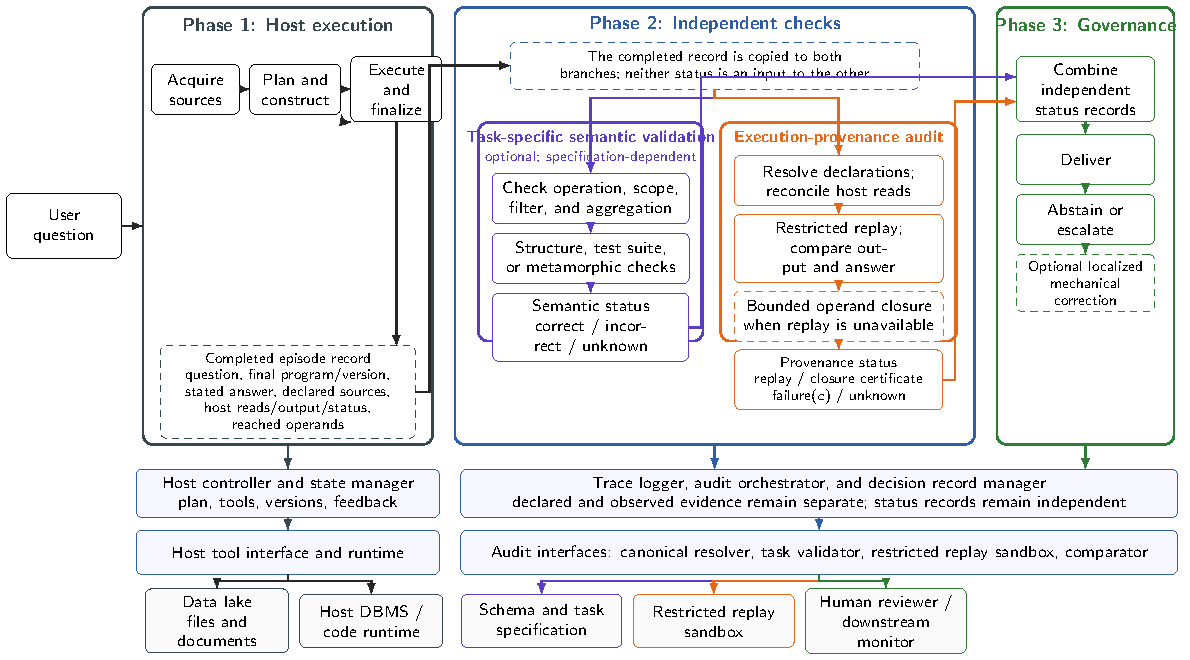
\includegraphics[width=0.99\textwidth]{fig_architecture.pdf}
\caption{LEDGER consumes a completed episode after host execution. Semantic validation and execution-provenance auditing run independently; dashed boxes denote the bounded fallback and an optional correction path that is not evaluated here.}
\label{fig:architecture}
\end{figure*}

\subsection{Overview and trace capture}

The host wrapper records program revisions, the final program snapshot, stdout, exceptions, declared citations, runtime data reads, accessed columns, and scalar operands reaching the final expression. Paths and dataset identifiers are canonicalized before comparison. Declared sources, host reads, and replay reads remain separate fields throughout the audit record.

For dataframe programs, operand attribution follows accessed columns and scalar values that reach the final expression. For SQL, the record stores relations, projected attributes, predicates, aggregates, and returned scalars. Each outcome carries a concise evidence string and the machine-readable artifact needed to reproduce it.

\subsection{Episode audit and failure precedence}\label{sec:auditproc}

Algorithm~\ref{alg:audit} implements the complete audit. Evidence-boundary failures take precedence over replay failures, which take precedence over output mismatch. When several violations are observed, the record preserves the full set and exposes the earliest class as the primary outcome. Closure is consulted only when no explicit failure has been observed and the final runtime is unavailable.

\begin{algorithm}[t]
\caption{LEDGER episode audit}
\label{alg:audit}
\begin{algorithmic}[1]
\Require episode $E$, resolver $R$, sandbox $H$, comparator $\operatorname{cmp}$, operations $\opset$, depth $d$
\State $F_{\mathrm{res}}\gets R(F_{\mathrm{decl}})$
\If{some declaration is unresolved}
  \State \Return $\failure(\mathrm{unresolved\ source})$
\EndIf
\If{$F_{\mathrm{host}}\nsubseteq F_{\mathrm{res}}$}
  \State \Return $\failure(\mathrm{undeclared\ host\ read})$
\EndIf
\If{$s_{\mathrm{host}}\neq\mathrm{success}$ and an answer was stated}
  \State \Return $\failure(\mathrm{host\ execution})$
\EndIf
\If{$P^*$ is runnable in $H$}
  \State $(F_{\mathrm{replay}},s_{\mathrm{replay}},v_{\mathrm{replay}})\gets\operatorname{Replay}(P^*,H[F_{\mathrm{res}}])$
  \If{$F_{\mathrm{replay}}\nsubseteq F_{\mathrm{res}}$}
    \State \Return $\failure(\mathrm{replay\ boundary})$
  \ElsIf{$s_{\mathrm{replay}}\neq\mathrm{success}$}
    \State \Return $\failure(\mathrm{replay\ execution})$
  \ElsIf{$v_{\mathrm{replay}}$ is not comparable}
    \State \Return $\failure(\mathrm{missing\ output})$
  \ElsIf{$\operatorname{cmp}(v_{\mathrm{replay}},\hat a;\tol)=1$}
    \State \Return $\cert_{\mathrm{replay}}$ and replay witness
  \Else
    \State \Return $\failure(\mathrm{output\ mismatch})$
  \EndIf
\EndIf
\If{reached operands are complete}
  \State \Return \Call{BoundedClosure}{$\operands,\opset,d,\hat a$}
\EndIf
\State \Return $\unknown$
\end{algorithmic}
\end{algorithm}

\subsection{Citation-restricted replay}

The replay sandbox mounts only $F_{\mathrm{res}}$, fixes deterministic library settings when available, and records every data read. The comparator normalizes strings, booleans, ordered or unordered lists, and numeric values under relative tolerance $\tol$. A successful certificate therefore binds a concrete program snapshot, a canonical evidence view, and a comparable output. Failure records retain the denied read, exception, missing output, or mismatching value that caused the decision.

\subsection{Operand-constrained fallback}\label{sec:closure}

Some archived episodes expose operands and a stated value while the original runtime is unavailable. Let
\[
\opset=\{\mathrm{sum,diff,ratio,pctchg,prod}\}.
\]
Starting from the trace-local operand multiset $\operands$, the depth-$d$ closure $\cl_d(\operands)$ recursively applies valid operations in $\opset$ with normalization and duplicate removal.

\begin{definition}[Closure certificate]\label{def:closure}
Episode $E$ receives a depth-$d$ closure certificate when $\hat a\in\cl_d(\operands)$ within tolerance $\tol$. The witness stores a minimal expression and its operand subset.
\end{definition}

\begin{algorithm}[t]
\caption{Bounded operand closure}
\label{alg:closure}
\begin{algorithmic}[1]
\Function{BoundedClosure}{$\operands,\opset,d,\hat a$}
\State $S_0\gets\operatorname{normalize}(\operands)$
\For{$j=1,\ldots,d$}
  \State $S_j\gets S_{j-1}$
  \ForAll{$x,y\in S_{j-1}$ and $o\in\opset$}
    \State add valid normalized $o(x,y)$ with an expression witness
  \EndFor
\EndFor
\If{$\hat a\in S_d$ within $\tol$}
  \State \Return $\cert_{\mathrm{closure}}$ and a minimal witness
\EndIf
\State \Return $\unknown$
\EndFunction
\end{algorithmic}
\end{algorithm}

\begin{proposition}[Closure completeness]\label{prop:complete}
If $\hat a$ is generated from reached operands by operations in $\opset$, expression depth at most $d$, and the audit's normalization and tolerance, then $\hat a\in\cl_d(\operands)$.
\end{proposition}
\noindent\emph{Proof sketch.} Leaves occur in $S_0$. Induction on expression depth places each valid internal result in the next closure level. The root therefore appears by depth $d$; The full proof appears in~\ref{app:proofs}.

The operating point is calibrated on 60 disjoint ConvFinQA examples and frozen at $d=2$ with relative tolerance $10^{-4}$. Context-wide numbers, held-out examples, and human labels do not change this setting.

\subsection{Semantic interface and governance decision}\label{sec:semanticinterface}

The audit record exposes $q$, $P^*$, schema references, and replay output to the optional validator $V_q$. SQL tasks permit normalized-structure comparison and execution on generated database variants \citep{zhong2020testsuite}; other deployments may supply executable constraints, metamorphic relations, a model-based judge, or human review. The resulting semantic status is appended to the audit record without modifying its provenance outcome.

A conservative decision policy delivers a provenance-certified answer when the semantic status is correct or unavailable under the deployment policy, and escalates semantically rejected or provenance-incomplete episodes. A uniquely localized mechanical mismatch can support an optional correction workflow; the present evaluation measures delivery and escalation and does not evaluate automated repair.



\begin{remark}
The provenance witness remains valid without a semantic validator. Semantic status is a separate, deployment-specific property.
\end{remark}

\subsection{Complexity and deterministic contract}

Resolution and read reconciliation cost $O(|F_{\mathrm{decl}}|+|F_{\mathrm{host}}|)$. Replay adds one execution of the final program. If $N_j$ is the number of closure candidates before duplicate removal, $m=|\operands|$, and $r=|\opset|$, then $N_d\le m+r\sum_{j=1}^{d}N_{j-1}^2$. Restricting $S_0$ to reached operands reduces every recursive expansion. For a fixed trace, resolver, runtime, comparator, normalization, and depth, the provenance audit is deterministic and invokes no language model.

\begin{table}[!t]
\centering
\caption{Interface between independent statuses and downstream action.}
\label{tab:policy}
\scriptsize
\begin{tabular}{@{}lll@{}}
\toprule
Provenance status & Semantic status & Default action \\
\midrule
certificate & correct & deliver \\
certificate & unknown & deliver or review by policy \\
certificate & incorrect & abstain / escalate \\
failure or unknown & any & abstain / escalate \\
localized mismatch & correct/unknown & optional correction \\
\bottomrule
\end{tabular}
\end{table}

% Requires \usepackage{placeins} in main.tex.

\section{Evaluation}
\label{sec:evaluation}

\subsection{Questions, evidence layers, and metrics}
\label{sec:setup}

We ask four questions.
\begin{description}
\setlength{\itemsep}{0pt}
\setlength{\parskip}{0pt}

\item[RQ1]
How does operand-constrained auditing compare with ordinary
numeric, trace-rule, anomaly, and model-based checks?

\item[RQ2]
Does the frozen audit transfer across datasets, and how does
closure depth expose its derivation--collision trade-off?

\item[RQ3]
Which semantic changes remain invisible to execution-result
equality, and which complementary checks detect them?

\item[RQ4]
Do replay certificates improve the quality of completed episodes
delivered to users or downstream systems?
\end{description}

\etitle{Evidence layers.}
ConvFinQA and MultiHiertt evaluate the bounded-closure component
using program-labelled numerical derivations and aligned
cross-example answer substitutions. WikiSQL evaluates the
task-specific semantic interface through controlled program
perturbations. KramaBench and DABstep evaluate completed
data-agent episodes through restricted replay, failure
localization, and selective delivery. The KramaBench human label
is a composite deliverability judgement: it asks whether the
stated answer follows from the cited data through the recorded
computation and addresses the requested quantity.

\begin{table}[t]
\centering
\caption{Evaluation layers and their primary roles. Size reports
total/evaluable instances where the distinction applies.}
\label{tab:datasets}
\scriptsize
\renewcommand{\arraystretch}{1.05}
\setlength{\tabcolsep}{2.5pt}
\begin{tabularx}{\columnwidth}{@{}l l r X@{}}
\toprule
Layer & Dataset & Size & Primary use \\
\midrule
Closure
& ConvFinQA
& 388/386
& Arithmetic audit and baselines \\

Closure
& MultiHiertt
& 7,830/6,301
& Transfer and depth stress \\

Semantic
& WikiSQL
& 500/2,715
& Same-output program changes \\

Live audit
& KramaBench
& 166
& Replay and selective delivery \\

Live audit
& DABstep
& 60
& Completed-episode transfer \\

Human
& KramaBench
& 40/39
& Deliverability and escalation \\
\bottomrule
\end{tabularx}
\end{table}

\etitle{Metrics.}
For program-labelled examples, \emph{reference-derivation recall}
is the fraction of supported derivations that receive a closure
certificate, and \emph{cross-example rejection} is the fraction
of aligned unsupported substitutions that do not receive one.
For WikiSQL, \emph{perturbation detection} is the fraction of
modified queries identified as changed, while the false-positive
rate is measured on unmodified reference queries. For selective
delivery, \emph{coverage} is the fraction of evaluable episodes
delivered; \emph{delivered support} is the fraction of delivered
episodes judged supported by human annotators;
\emph{supported-case retention} is the fraction of all
human-supported episodes retained; and \emph{mean delivered
score} averages the benchmark's official score over delivered
episodes.

\etitle{Baselines.}
Numeric baselines include exact operand matching, one-operation
derivability, and closure over all numbers in the cited context.
Trace rules check execution success, citation resolution,
declared-read coverage, and unrestricted replay. Anomaly baselines
use robust MAD distance, Isolation Forest
\citep{liu2008isolation}, Local Outlier Factor
\citep{breunig2000lof}, and one-class SVM
\citep{scholkopf2001support}. Their thresholds use only the
60-example calibration seed and retain at least 90\% supported
derivations on that seed. A supervised logistic model provides an
upper baseline. No anomaly feature contains the audit verdict or
benchmark answer.

\etitle{Evidence-aware judge.}
A local Qwen3.6-35B judge receives the question, declared evidence
metadata, observed reads, program summary, execution status,
recomputed output, and stated answer. It receives neither benchmark
gold nor \ledger labels. Three temperature-zero repeats measure
response stability. Transferred human records omit most raw rows
and complete program bodies, so that subset remains a
limited-evidence diagnostic.

\subsection{RQ1: Program-reached operands separate derivations
from numeric coincidence}
\label{sec:rq1}

\begin{figure*}[!t]
\centering
\begin{minipage}[t]{0.316\textwidth}
\centering
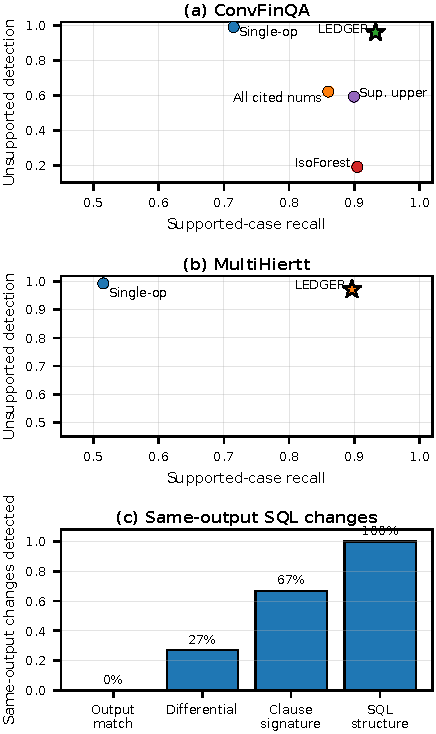
\includegraphics[
  width=\linewidth,
  trim=0 234.8bp 0 0,
  clip
]{fig_baselines_semantics_3panel.pdf}
\end{minipage}
\hfill
\begin{minipage}[t]{0.316\textwidth}
\centering
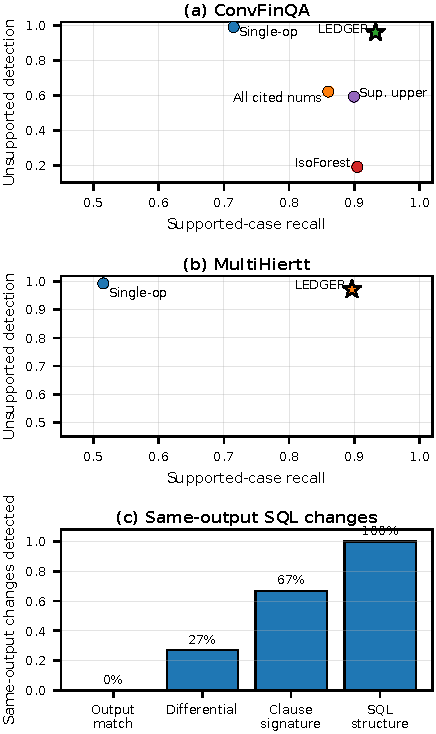
\includegraphics[
  width=\linewidth,
  trim=0 117.4bp 0 117.4bp,
  clip
]{fig_baselines_semantics_3panel.pdf}
\end{minipage}
\hfill
\begin{minipage}[t]{0.316\textwidth}
\centering
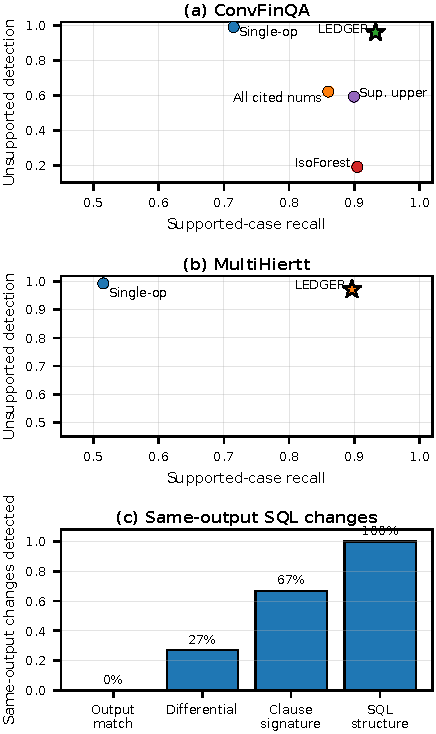
\includegraphics[
  width=\linewidth,
  trim=0 0 0 234.8bp,
  clip
]{fig_baselines_semantics_3panel.pdf}
\end{minipage}
\caption{%
Operand-constrained auditing on ConvFinQA and MultiHiertt,
together with the semantic complement on WikiSQL.
Panels (a,b) report reference-derivation recall and
cross-example rejection; panel (c) reports detection on
same-output SQL changes.}
\label{fig:baselines}
\end{figure*}

\etitle{Trace-local closure preserves derivations and suppresses
unrelated numbers.}
ConvFinQA supplies 386 evaluable reference derivations and aligned
cross-example substitutions; MultiHiertt supplies 6,301 aligned
pairs. The frozen checker uses program-reached operands, five
operations, depth 2, and relative tolerance $10^{-4}$. It recovers
93.3\% and 89.6\% of the reference derivations on ConvFinQA and
MultiHiertt, while rejecting 96.1\% and 97.2\% of the corresponding
cross-example substitutions. Closure over all cited-context
numbers recovers additional derivations over one-operation
checking, but also admits many unrelated numeric coincidences.

\begin{table}[t]
\centering
\caption{ConvFinQA baselines on the held-out remainder.}
\label{tab:baselines}
\scriptsize
\setlength{\tabcolsep}{3pt}
\begin{tabular}{@{}lcc@{}}
\toprule
Method
& Derivation recall
& Cross-example rejection \\
\midrule
Single operation
& 276/386 (0.715)
& 383/386 (0.992) \\

All cited numbers
& 332/386 (0.860)
& 240/386 (0.622) \\

Isolation Forest
& 351/388 (0.905)
& 74/388 (0.191) \\

Supervised upper
& 349/388 (0.899)
& 230/388 (0.593) \\

\textbf{\ledger}
& \textbf{360/386 (0.933)}
& \textbf{371/386 (0.961)} \\
\bottomrule
\end{tabular}
\end{table}

\etitle{Standard anomaly scores do not produce a derivation
witness.}
Isolation Forest, Local Outlier Factor, and one-class SVM retain
most supported examples but reject only 13.7--19.8\% of the
cross-example substitutions. Their trace features identify unusual
executions, but do not establish that the answer follows from the
program-reached values. Restricting closure to those operands
preserves the relevant search space and removes unrelated context
numbers before recursive expansion.

\subsection{RQ2: Closure depth recovers derivations and expands
the collision surface}
\label{sec:rq2}

\begin{figure}[!t]
\centering
\begin{minipage}[t]{0.49\columnwidth}
\centering
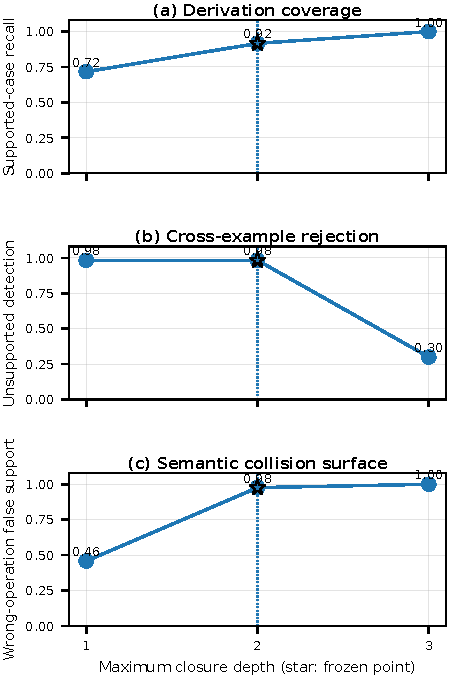
\includegraphics[
  width=\linewidth,
  trim=0 216.8bp 0 0,
  clip
]{fig_depth_ablation_3panel.pdf}
\end{minipage}
\hfill
\begin{minipage}[t]{0.49\columnwidth}
\centering
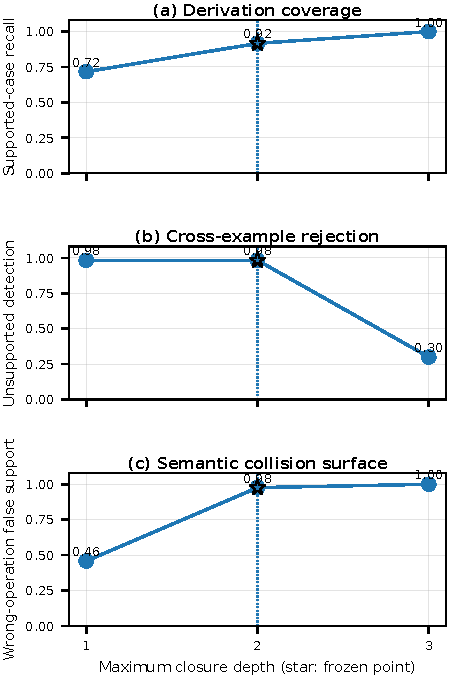
\includegraphics[
  width=\linewidth,
  trim=0 108.4bp 0 108.4bp,
  clip
]{fig_depth_ablation_3panel.pdf}
\end{minipage}

\vspace{1pt}

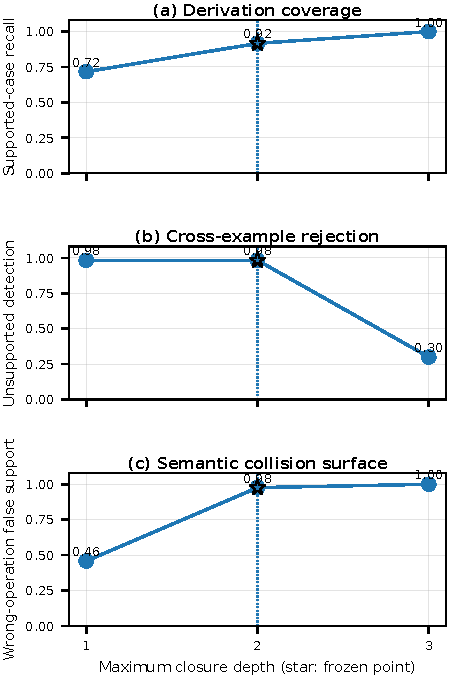
\includegraphics[
  width=0.72\columnwidth,
  trim=0 0 0 216.8bp,
  clip
]{fig_depth_ablation_3panel.pdf}
\caption{%
Effect of closure depth on derivation coverage,
cross-example rejection, and wrong-operation false support.
The star marks the frozen depth-2 setting.}
\label{fig:ablation}
\end{figure}

\etitle{Depth 2 captures short programs while retaining
cross-example rejection.}
We stratify MultiHiertt by reference-program depth and vary closure
depth on the disjoint ConvFinQA calibration seed. Most remaining
MultiHiertt misses correspond to programs deeper than the frozen
bound: 72.3\% of misses exceed depth 2. Increasing calibration
depth from 1 to 3 recovers every supported seed derivation, while
cross-example rejection falls sharply
(Figure~\ref{fig:ablation}a,b).

\etitle{Additional depth enlarges the semantic collision surface.}
We replace each ConvFinQA answer with the result of a different
operation over the same operands. Across all 382 substitutions,
only 9 are rejected; none of the 347 substitutions within the
frozen operation vocabulary and depth is rejected. Deeper closure
accepts still more variants because the altered answers remain
derivable from the same values
(Figure~\ref{fig:ablation}c). Closure therefore records arithmetic
derivability, while operation identity remains a semantic property.

\subsection{RQ3: Structural validation detects same-output
program changes}
\label{sec:rq3}

\etitle{Execution-result equality misses semantic changes.}
From 500 executable WikiSQL development examples, we construct
2,715 perturbations that alter aggregation, projection, predicate
column or value, or predicate presence. Execution-result equality
misses 466 perturbations because the modified and reference
programs return the same result on the original database.

\etitle{Program structure complements replay.}
Normalized SQL structure detects all 2,715 perturbations with no
false positives on the 500 unmodified reference queries. On a
100-case same-output sample, operator/clause signatures detect
67 changes and differential execution detects 27, while
original-database output comparison detects none
(Figure~\ref{fig:baselines}c). Structural comparison observes the
changed program directly; execution on database variants succeeds
when the variants separate the candidate and reference programs.
SQL deployments can therefore instantiate $V_q$ through structural
and test-suite methods \citep{zhong2020testsuite}; model-based
metrics such as FLEX remain an alternative when reference programs
are unavailable \citep{kim2025flex}.

\subsection{RQ4: Replay certificates support selective delivery}
\label{sec:rq4}

\begin{figure}[!t]
\centering
\begin{minipage}[t]{0.49\columnwidth}
\centering
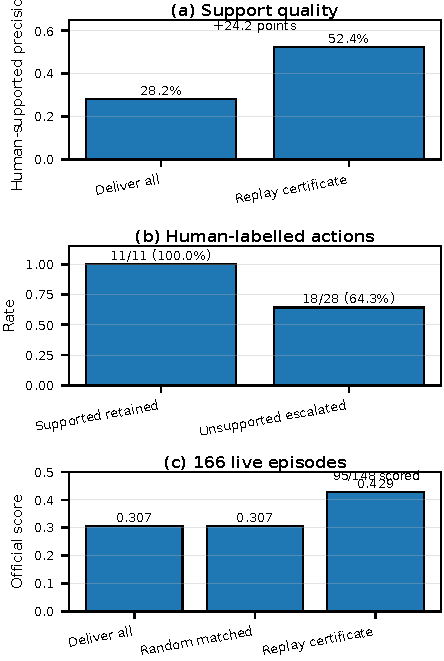
\includegraphics[
  width=\linewidth,
  trim=0 211.5bp 0 0,
  clip
]{fig_governance_3panel.pdf}
\end{minipage}
\hfill
\begin{minipage}[t]{0.49\columnwidth}
\centering
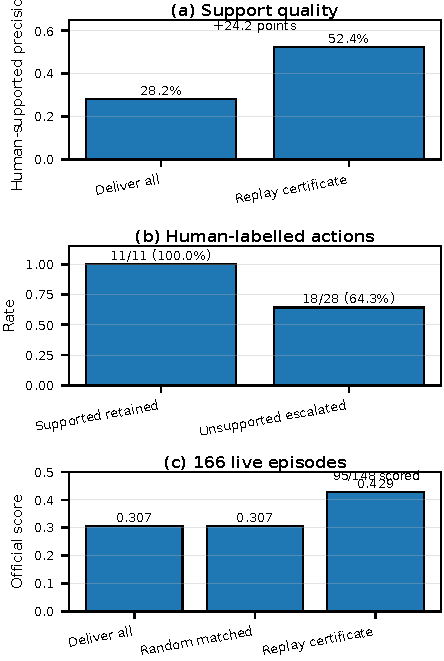
\includegraphics[
  width=\linewidth,
  trim=0 105.7bp 0 105.7bp,
  clip
]{fig_governance_3panel.pdf}
\end{minipage}

\vspace{1pt}

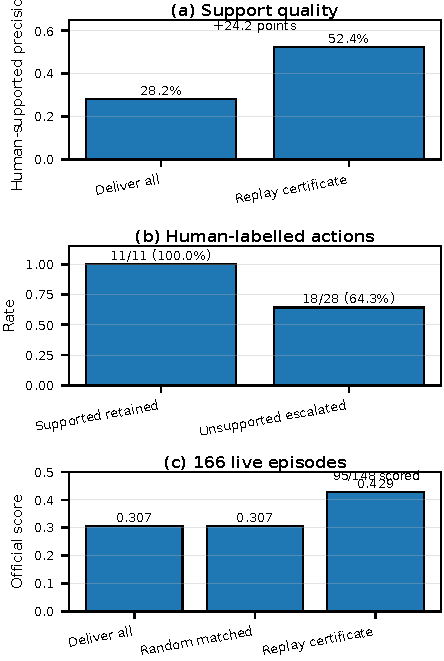
\includegraphics[
  width=0.72\columnwidth,
  trim=0 0 0 211.5bp,
  clip
]{fig_governance_3panel.pdf}
\caption{%
Replay-based selection improves delivered support, retains
human-supported episodes, escalates unsupported episodes, and
raises mean delivered score at partial coverage.}
\label{fig:governance}
\end{figure}

\etitle{Replay status provides a human-facing delivery signal.}
The live corpus contains 166 KramaBench and 60 DABstep episodes.
Among 39 KramaBench episodes with clear human labels, delivering
only replay-certified episodes retains all 11 supported cases and
escalates 18 of 28 unsupported cases. The proportion of delivered
answers judged supported consequently rises from 28.2\% to 52.4\%
(Figure~\ref{fig:governance}a,b). The remaining replay-certified
but human-unsupported episodes reproduce a value through programs
that address the wrong quantity, scope, or operation, consistent
with the separation between provenance and semantics.

\etitle{The same certificate improves score at partial coverage.}
Among 148 KramaBench episodes with finite official scores,
replay-certificate delivery selects 95 episodes, corresponding to
64.2\% coverage. Their mean official score is 0.429, compared with
0.307 for delivering all episodes and 0.307 for uniformly random
selection at the same size
(Figure~\ref{fig:governance}c). The policy changes which completed
episodes are delivered; it does not modify host-agent source
selection, program generation, or execution.

\subsection{Runtime, determinism, and model baseline}
\label{sec:runtime}

\etitle{Deterministic bookkeeping is small relative to host
execution.}
Across 500 saved records, the audit adds sub-millisecond median
bookkeeping and makes zero model calls. Five independent repeats
over 100 records produce identical execution-provenance outcomes.
These measurements cover record parsing, comparison, and closure
over saved traces; they exclude host-agent execution and external
data loading.

\etitle{The model judge remains a diagnostic baseline.}
An evidence-aware 35B judge shows label disagreement,
structured-output failures, and occasional repeat flips. The
complete counts appear in Appendix~\ref{app:tables}. Judge outputs
do not alter the deterministic execution-provenance status.

% \FloatBarrier
\section{Related Work}\label{sec:related}

\paragraph{Data-agent evaluation.}
KramaBench evaluates data-to-insight pipelines over heterogeneous lake files \citep{kramabench2025}; DABstep targets multi-step tool-based analysis \citep{dabstep2025}. LakeQA scales discovery and reasoning to a million-scale lake \citep{lakeqa2026}. SANA decomposes failures across search, planning, analysis, and policy \citep{sana2026}. These benchmarks motivate process-level evidence in addition to final-answer accuracy.

\paragraph{Execution provenance and auditability.}
Database provenance formalizes how outputs depend on inputs \citep{green2007provenance,cheney2009provenance,amsterdamer2011aggregate}. noWorkflow and Vamsa capture dependencies in data-science scripts \citep{murta2014noworkflow,namaki2020vamsa}. Agent-trace work organizes retrieved evidence, tool outputs, memory, actions, and final claims under process-level accountability \citep{agenttrace2026}. Auditable Agents distinguishes accountability, auditability, and auditing and identifies action recoverability and evidence integrity as core dimensions \citep{nian2026auditable}. \ledger operationalizes these dimensions for completed computed answers and their declared evidence view.

\paragraph{Agent governance, security, and trace evaluation.}
Contextual security frameworks separate task alignment, action alignment, source authorization, and data isolation \citep{siu2026security}; intent-to-execution integrity further separates tool, instruction, judgment, and data-flow properties \citep{qu2026intent}. The provenance status in \ledger covers an observed source and execution boundary, while its task-specific semantic interface addresses a separate alignment relation. TrustAgent intervenes before, during, and after planning through an agent constitution \citep{hua2024trustagent}; \ledger instead audits a completed episode. ToolEmu, AgentDojo, and R-Judge establish tool trajectories as standard evaluation objects \citep{ruan2024toolemu,debenedetti2024agentdojo,yuan2024rjudge}.

\paragraph{Citation, semantic, and selective evaluation.}
ALCE and FActScore evaluate textual citation support and factual claims \citep{gao2023alce,min2023factscore}. Text-to-SQL test suites approximate semantic equivalence through execution on multiple database variants \citep{zhong2020testsuite}; FLEX uses an LLM-based expert metric to reduce execution-metric errors \citep{kim2025flex}. Selective QA trades coverage for reliability using confidence \citep{kamath2020selective}. \ledger derives its delivery signal from a replay witness and retains task-specific semantic evaluation as an independent control.

\section{Limitations}\label{sec:limitations}

The guarantee is relative to the trusted logger, resolver, sandbox, and comparator. Tamper-evident logging, sandbox escape, nondeterministic network services, and unobserved dependencies remain outside the current threat model. Platform-level controls are needed before the same certificate semantics can be applied in adversarial environments.

The arithmetic fallback supports a frozen five-operation vocabulary and depth 2. It omits string transformations, joins, and long programs when replay is unavailable. Increasing depth improves derivation coverage and rapidly increases collisions. Current replay adapters cover the Python/pandas and SQL traces retained by the testbed families; additional formats require runtime-specific adapters.

Human support is available for 39 clear KramaBench cases. A larger independently annotated corpus would strengthen estimates of deployment prevalence. The WikiSQL study uses controlled perturbations and access to reference programs. It demonstrates the complementarity of replay and structural validation; it does not establish universal natural-language-to-program equivalence. Automated mechanical correction is shown only as a downstream interface and is not evaluated in this paper.

\section{Conclusion}\label{sec:conclusion}

Computed data-agent answers require evidence that spans declared sources, observed reads, final programs, execution outcomes, and stated values. \ledger converts a completed episode into a deterministic execution-provenance record through source resolution, read reconciliation, citation-restricted replay, and bounded operand closure. Ordinary rules and anomaly detectors do not match its joint derivation recall and unsupported-answer detection. Live traces show that replay certificates support selective delivery while preserving an explicit unknown path. Controlled SQL perturbations establish the complementary role of task-specific semantic validation. Together, the two independent statuses provide a reproducible basis for delivery and escalation decisions.


\appendix
\section{Proofs}\label{app:proofs}

\subsection{Theorem~\ref{thm:relative}}
A replay certificate is returned only after every declaration resolves, both observed read sets lie within the resolved evidence view, host and replay execution succeed, and the frozen comparator matches replay output to the stated answer. Under the trust assumptions, these observations correspond to the recorded data dependencies and the sandbox-enforced execution. Each listed violation negates at least one required conjunct in Equation~\ref{eq:replaycert} and follows a failure branch in Algorithm~\ref{alg:audit}; hence no replay certificate is returned.

\subsection{Proposition~\ref{prop:complete}}
At depth zero, every leaf is a reached operand and belongs to $S_0$. Assume every valid expression of depth at most $j-1$ is represented in $S_{j-1}$. An expression of depth $j$ has the form $o(e_1,e_2)$ with $o\in\opset$ and child depth at most $j-1$. The induction hypothesis places both child values in $S_{j-1}$; Algorithm~\ref{alg:closure} adds their valid normalized result to $S_j$. The root therefore appears by depth $d$.

\subsection{Proposition~\ref{prop:semantic}}
Replay compares the submitted program's output with the stated answer under the declared evidence view. Closure tests whether the answer has an admitted derivation from reached operands. Neither predicate compares the submitted program with $V_q$. Choose two programs with different task semantics but identical output on the current database, or two different admitted arithmetic expressions with the same result. The provenance predicate holds while the semantic validator rejects the altered program.

\section{Additional Result Tables}\label{app:tables}

\begin{table}[ht]
\centering
\caption{Canonical live audit distributions.}
\scriptsize
\begin{tabular}{@{}lrrrr@{}}
\toprule
Dataset & Total & Replay & Failure & Unknown \\
\midrule
KramaBench & 166 & 107 & 3 & 56 \\
DABstep & 60 & 43 & 0 & 17 \\
\bottomrule
\end{tabular}
\end{table}

\begin{table}[ht]
\centering
\caption{Evidence-aware local judge. Agreement uses construction or human labels; the human row has limited archived evidence.}
\scriptsize
\begin{tabular}{@{}lrrr@{}}
\toprule
Dataset & Agreement & Flip items & Parse failures \\
\midrule
ConvFinQA constructed & 170/200 & 4/200 & \multirow{3}{*}{29/870} \\
KramaBench human & 25/39 & 1/39 & \\
WikiSQL perturbations & 44/50 & 3/50 & \\
\bottomrule
\end{tabular}
\end{table}

\section{Human Annotation and Reproducibility}\label{app:human}

The 40-row sample spans archeology, environment, legal, and wildfire domains. Annotators receive the question, cited files, final program or available program summary, stated answer, replay output, and evidence notes. The support label asks whether the stated answer follows from the cited data through the recorded computation and whether that computation addresses the requested quantity. The benchmark answer and machine label are hidden. Labels are yes, no, and unclear; one unclear case is excluded from binary analysis.

Machine outputs are frozen before annotation. Human columns remain in a separate file and are never used to rewrite audit labels. The reproducibility package contains the operating point, per-example arithmetic records, live trace records, semantic perturbations, baseline scripts, figure-generation code, and SHA-256 manifests. Every rate in the paper is recoverable from machine-readable counts.

\section*{Declaration of generative AI and AI-assisted technologies in the writing process}
During the preparation of this work, the authors used OpenAI ChatGPT to assist with manuscript restructuring, language editing, figure preparation, and LaTeX preparation. The authors reviewed and edited the resulting content and take full responsibility for the publication.


\bibliographystyle{elsarticle-num}
\bibliography{refs}

\end{document}
